\clearpage
%%%%%%%%%%%%%%%%%%%%%%%%%%%%%%%%%%%%%%%%%%%%%%%%%%%%%%%%%%%%%%%%%%%%%%%%%%%%%%%
\section{Week 0: Ray Tracing Class}
%%%%%%%%%%%%%%%%%%%%%%%%%%%%%%%%%%%%%%%%%%%%%%%%%%%%%%%%%%%%%%%%%%%%%%%%%%%%%%%

\subsection*{Thursday, 06/13/2023}
\begin{itemize}
    \item \textcolor{DarkGreen}{\href{https://raytracing.github.io/books/RayTracingInOneWeekend.html}{course link}}
    \item shoutout to \textbf{\textcolor{Maroon}{TODO}} add x user that pointed
        me to this (shoutout ml btw (for you page))
        % todo add twitter user whomst this is from
    \item this is my very first c or cpp project (op says it's c flavored cpp) 
        beyond hello worlds and basic basic robotics stuff
    \item i love rust but i am not cracked at all so i would probably not be
        able to follow along in rust
    \item i will, however, follow op's advice to not copy pasta (besides most of 
        makefile compiler flags hehehe) and build it up slowly by typing along
    \item going to try my best to thug this out by Sunday
    \item test bib \cite{Shirley2024RTW1}
    \item bib working lets go
    \item important setup for fresh arch install (not in order, and just off the
        dome, i likely am forgetting tons of things)
        \begin{itemize}
            \item install unzip (will need for nvim clangd Mason lsp stuff)
            \item install cmake, clangd, gcc stuff
            \item setup debugger for nvim using dap, dap-ui, etc. 
            \item \textbf{build, compile, run:} (i think lol)
                \begin{enumerate}
                    \item \texttt{cmake -B build/Debug -DCMAKE_BUILD_TYPE=Debug} 
                    \item \texttt{cmake --build build/Debug} 
                    \item \texttt{build/rayTracing > image.ppm} 
                \end{enumerate}
        \end{itemize}
    \item op claims that if we can build project correctly in the beginning,
        then we are golden for rest of tutorial
    \item i hope this is true since the provided cmake file is cash money and
        really easy to get working with my setup
        (Figure~\ref{fig:rt_weekend_main_build_success})
    \item make \texttt{rtrace} aliase for build, compile, run, then open image
        in feh, probably terrible idea but whatever 
    \item got color header file with a \texttt{write_color} util function
    \item now working on a \texttt{ray} class which will use our \texttt{vec3} 
        class.
    \item refresher on rays: think of them as functions 
        (Equation~\ref{eq:rays}):
        \begin{equation}
            \mathbf{P}(t) = \mathbf{A} + t\mathbf{b}
            \label{eq:rays}
        \end{equation}
    \item here $\mathbf{P}$ is a 3D position along a line in 3D. $\mathbf{A}$ is
        the ray origin and $\mathbf{b}$ is the ray direction. The ray parameter
        $t$ is a real number (\texttt{double} in the code). Plug in a different
        $t$ and $\mathbf{P}(t)$ moves the point along the ray. Add in negative t
        values and you can go anywhere on the 3D line. For positive $t$, you get
        only the parts in front of $\mathbf{A}$, and this is what is often
        called a half-line or a ray. (Figure~\ref{fig:linear_interpolation}) 
        \begin{figure}[ht]
            \centering
            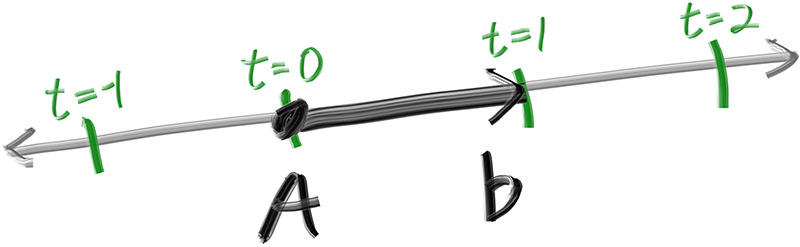
\includegraphics[width=12cm]{linear_interpolation}
            \captionsetup{labelfont=bf, textfont=it}
            \caption{linear interpolation}
            \label{fig:linear_interpolation}
        \end{figure}
    \item  ...
\end{itemize}
